\documentclass[12pt, a4paper]{ctexart}
\usepackage{amsmath, amsthm, amssymb, appendix, bm, graphicx, hyperref, mathrsfs}
\usepackage{indentfirst} % 用于开头空两格
\usepackage{pifont} % 用于显示圆标数字
\usepackage{minted} % 设置行内代码
\usepackage{listings} % 插入代码用到
\usepackage{pythonhighlight} % python代码高亮
%% 用于子图
\usepackage{subfigure}
\usepackage{parskip}
%% 用于写算法
\usepackage{algorithm}
\usepackage{algorithmic}
\renewcommand{\algorithmicrequire}{ \textbf{Input:}} %Use Input in the format of Algorithm
\renewcommand{\algorithmicensure}{ \textbf{Output:}} %UseOutput in the format of Algorithm
%% 用于设置itemize间距
\usepackage{enumitem}
\setenumerate[1]{itemsep=0pt,partopsep=0pt,parsep=\parskip,topsep=5pt}
\setitemize[1]{itemsep=0pt,partopsep=0pt,parsep=\parskip,topsep=5pt}
\setdescription{itemsep=0pt,partopsep=0pt,parsep=\parskip,topsep=5pt}
%% 用于设置边距
\usepackage{geometry}
\geometry{left=2cm,right=2cm,top=2cm,bottom=2cm}

\title{\textbf{智能推荐系统第一次作业报告}\\
Memory-based CF for Rating Prediction}
\author{宋朝芸 10215001419}
\date{\today}
\linespread{1.5}


\begin{document}

\maketitle

\setcounter{page}{0}
\maketitle
\thispagestyle{empty}


\pagenumbering{Roman}
\setcounter{page}{1}
\tableofcontents
\newpage
\setcounter{page}{1}
\pagenumbering{arabic}

\section{算法介绍}

\subsection{协同过滤算法概述}


基于记忆的协同过滤算法(Memory-based Collaborative Filtering)是一种基础的推荐算法。这种算法没有可学习的参数,使用近邻用户和物品的统计信息进行推荐。一般可以将近邻集合的评分根据相似度加权平均得到预测值。因此,算法的要点为:
\begin{itemize}
    \item 计算相似度
    \item 确定近邻集合
    \item 使用相似度和近邻集合进行评分预测
\end{itemize}


\textbf{1. 相似度计算}

根据相似度的计算对象,算法可以分为两种类型:\ding{192}基于用户的协同过滤(user-based CF),\ding{193}基于物品的协同过滤(item-based CF)。

其中,user-based CF能够反映物品在用户小圈子中的流行度,适用场景如新闻推荐,并且适合物品数量远大于用户数量的情况;item-based 能够反映用户自身偏好,适用场景如电影推荐,且适合用户数量远大于商品数量。

根据相似度的计算方法,主要分为以下几种类型:\ding{192}Pearson相关系数,\ding{193}Jaccard系数,\ding{194}余弦相似度,\ding{195}MSE相似度.

此外,还可以对计算得到的所有相似度进一步处理:\ding{192}中心化(减去用户或物品的平均评分),\ding{193}z score标准化,\ding{194}01归一化。

\textbf{2. 近邻集合确定}

确定近邻集合,可以分为以下几种方法:\ding{192}给定集合大小$K$(top-K或随机选择),\ding{194}给定相似度阈值$\lambda$,\ding{195}全集,\ding{196}聚类结果属于同一类。

\textbf{3. 预测评分}

进行评分预测,最主要的方法是将近邻集合中每一项的评分使用相似度进行加权平均,也可以考虑直接平均或多元线性回归模型。

此外,改进的方法还包括:\ding{192}加入流行度的计算,在加权时对流行度高的评分进行惩罚,\ding{193}考虑时间衰减因素,在加权时对时间久远的相似性进行惩罚,\ding{194}加入方差的计算,在加权时对方差更大的评分以更高的权重。

\subsection{所用算法描述}

本次实验主要采用基于用户的协同过滤算法,以Pearson相关系数作为相似度,给定大小的top-K确定近邻集合,使用相似度加权平均预测评分。算法见Algorithm 1.

\begin{algorithm}[htb] 
\caption{user-based CF}
\label{alg:Framwork} 
\begin{algorithmic} 
\REQUIRE ~~\\ %算法的输入参数:Input
用户集合$U$,物品集合$I$,稀疏评分矩阵$R$,相似度阈值$\lambda$,近邻集合大小$K$,要预测的用户$u$和物品$i$,其中$u\in U,i \in I$.
\ENSURE ~~\\ %算法的输出:Output

\STATE 1. 对于所有用户$v\neq u$,计算相似度$w_{u,v}$:
\STATE 对于用户$v$,计算用户$u$和用户$v$共同评分过的商品集合P,然后计算$u$和$v$评分向量的Pearson相关系数:
$$w_{u,v} = 
\frac{\sum_{i\in P}{(r_{u,i} - \bar{r_u})(r_{v,i} - \bar{r_v})}}
{
\sqrt{\sum_{i\in P}{(r_{u,i} - \bar{r_u})}^2}
\sqrt{\sum_{i\in P}{(r_{v,i} - \bar{r_v})}^2}
}$$
\STATE 2.选择近邻集合$V\subset U$,集合$V$满足:
\STATE \ding{192}\ $\forall v \in V,w_{u,v}\geq \lambda$(相似度大于阈值),
\STATE \ding{193}\ $\lvert V\lvert\leq K$(近邻集合大小不超过给定大小),
\STATE \ding{194}\ $\forall v \in V,\forall x \not\in V, w_{u,v}\geq w_{u,x}$(近邻集合中的元素是和u最相似的),
\STATE \ding{195}\ $\forall v \in V,\exists r_{v,i}$(近邻集合中的元素对i有过评分).
\STATE 3. 计算预测值$s(u,i)$:
$$s(u,i)=\bar{r_u}+
\frac{\sum_{v\in V}{(r_{v,i} - \bar{r_v})*w_{u,v}}}
{\sum_{v\in V w_{u,v}}+1}$$

\RETURN $s(u,i)$; %算法的返回值
\end{algorithmic}
\end{algorithm}

此外,为了测试在同样使用Pearson相关系数的情况下不同相似度计算对象的效果,还稍作修改得到了item-based CF,具体算法见Algorithm 2.

\begin{algorithm}[htb] 
\caption{item-based CF}
\label{alg:Framwork} 
\begin{algorithmic}
\REQUIRE ~~\\ %算法的输入参数:Input
用户集合$U$,物品集合$I$,稀疏评分矩阵$R$,相似度阈值$\lambda$,近邻集合大小$K$,要预测的用户$u$和物品$i$,其中$u\in U,i \in I$.
\ENSURE ~~\\ %算法的输出:Output

\STATE 1. 对于所有物品$j\neq ui$,计算相似度$w_{i,j}$:
\STATE 对于物品$j$,计算物品$i$和物品$j$被共同评分过的用户集合C,然后
$$w_{i,j} = 
\frac{\sum_{u\in C}{(r_{u,i} - \bar{r_i})(r_{u,j} - \bar{r_j})}}
{
\sqrt{\sum_{u\in C}{(r_{u,i} - \bar{r_i})}^2}
\sqrt{\sum_{u\in C}{(r_{u,j} - \bar{r_j})}^2}
}$$
\STATE 2.选择近邻集合$J\subset I$,集合$J$满足:
\STATE \ding{192}\ $\forall j \in J,w_{i,j}\geq \lambda$(相似度大于阈值),
\STATE \ding{193}\ $\lvert J\lvert\leq K$(近邻集合大小不超过给定大小),
\STATE \ding{194}\ $\forall j \in J,\forall x \not\in V, w_{i,j}\geq w_{i,x}$(近邻集合中的元素是和i最相似的),
\STATE \ding{195}\ $\forall j \in J,\exists r_{u,j}$(近邻集合中的元素对i有过评分).
\STATE 3. 计算预测值$s(u,i)$:
$$s(u,i) =
\begin{cases}
\frac{\sum_{j\in J}{r_{u,j}*w_{i,j}}}{\sum_{j\in J} w_{i,j}}, & \text{if } \sum_{j\in J} w_{i,j} \neq 0 \\
\bar{r_i}, & \text{otherwise}
\end{cases}$$

\RETURN $s(u,i)$; %算法的返回值
\end{algorithmic}
\end{algorithm}

\newpage
\section{代码说明}

\subsection{环境与依赖}
本次实验的编程语言是Python 3.10.10,所用库包括:
\begin{itemize}
    \item pandas 2.0.1
    \item numpy 1.24.3
    \item sklearn 1.3.0(用于计算RMSE)
    \item surprise 1.1.3(用于划分测试集和验证集)
    \item matplotlib 3.7.1
\end{itemize}

\subsection{代码思路}

代码的总体思路分为模型选择和结果预测两步。

模型选择时,将\textbf{训练数据}划分为\textbf{测试集}和\textbf{验证集},在\textbf{训练集}上计算相似度矩阵和每位用户的评分,在\textbf{验证集}上选择合适的相似度阈值$\lambda$和近邻集合大小$K$。

结果预测时,使用选定的$\lambda,K$,在所有\textbf{训练数据}上计算相似度矩阵和每位用户的评分,并在\textbf{测试数据}上输出预测结果。

所用的主要函数如下:

\begin{itemize}
    \item 加载并划分数据 \verb|`load_and_split`|
    \item 计算验证集上的RMSE  \verb|`RMSE_calculate`|
    \begin{itemize}
        \item 计算基于Pearson相关系数的相似度矩阵 \verb|`pearson_sim_matrix`|
        \item 计算一对(user,item)的预测结果 \verb|`predict_rate`|
        \begin{itemize}
            \item 对给定的user和item选择近邻矩阵 \verb|`select_neighbor`|
        \end{itemize}
    \end{itemize}
    \item 对测试集输出预测 \verb|`predict_testset`|
\end{itemize}

\subsection{核心代码}
下以user-based CF为例解释代码,item-based基本只需要对user-item矩阵进行转置。
\subsubsection{load\_and\_split}

首先读取训练数据和测试数据文件。为了直观性,将训练数据转为user-item评分矩阵,以pandas数据框的形式存储。
\begin{python}
def load_and_split(train_path, test_path, size=0.2, state=None, choice = 0):
  # 加载csv数据集为pd数据框
  train = pd.read_csv(train_path)
  test = pd.read_csv(test_path)
  # 转为user-item矩阵
  train_df = train.pivot(index='userid',columns='itemid',values=['rate'])    
\end{python}

由于矩阵稀疏,为了便于计算RMSE的估计值,希望测试集和验证集都不丢失user和item的信息,因此使用surprise库划分数据。而surprise库只明确输出验证集,训练集无法使用,因此还需要遍历验证集来手动获取划分结果。

最后,为了使模型选择和结果预测两步能够复用该函数,增加选项choice变量。该变量取0表示模型选择,取1表示结果预测。

\begin{python}
  # 模型选择步
  if (choice == 0):
    # 加载pd数据框用于surprise包
    reader = Reader(rating_scale=(1, 10))
    load_train = Dataset.load_from_df(train, reader)
    # surprise包进行数据划分
    _, validset = train_test_split(load_train, test_size=size, random_state=state)

    train_set = train_df.copy()
    # 遍历validset,更新train_set = train_df - validset
    for row in validset:
        userid, itemid, rate = row
        # 在train_set中将valid_set中出现的值设为nan
        train_set.iloc[userid, itemid] = float('nan')
    
    return train_set, validset, test
    
  # 结果预测步
  if(choice == 1):
     return train_df, test
\end{python}


\subsubsection{pearson\_sim\_matrix}

计算用户之间的评分相似度时,要注意只能保留两个用户共同评分的物品,而pandas库的\verb|`.corr()`|恰好提供了一个快速且满足要求的方式,无需再计算共同评分过的物品集合P。注意在\verb|`load_and_split`|函数中,数据被转化为user-item评分矩阵,因此计算用户相似度之前需要对评分矩阵进行转置。

\begin{python}
def pearson_sim_matrix(dat):
  temp = dat.transpose()
  return temp.corr()
\end{python}


\subsubsection{select\_neighbor}

算法中要求近邻集合满足:\ding{192}\ $\forall v \in V,w_{u,v}\geq \lambda$,\ding{193}\ $\lvert V\lvert\leq K$,\ding{194}\ $\forall v \in V,\forall x \not\in V, w_{u,v}\geq w_{u,x}$,\ding{195}\ $\forall v \in V,\exists r_{v,i}$.为此,先用\verb|`np.where()`|筛选出大于阈值的用户,再遍历以筛选出对物品i有过评分的用户,然后使用\verb|`.sort()`|将相似度从大到小排序,最后获取前k个元素。由于需要近邻集合中的用户user、评分rating、相似度sim、用户均分mean,在遍历时就把这些信息一起存储到列表中,在函数末尾一起返回。

\begin{python}
def select_neighbor(dat, uid, iid, k, thres, mean, sim):  
  # 获取与用户u相似度大于阈值的用户列表
  neighbors = np.where(sim[uid] > thres)[0]
  # 获取对商品i评分过的用户列表及其对应的评分和相似度
  neighbors_info = [(v, dat.iloc[v, iid], sim.iloc[uid, v], mean.iloc[v]) for v in neighbors if not np.isnan(dat.iloc[v, iid])]
  # 根据与用户u的相似度降序排序
  neighbors_info.sort(key=lambda x: x[2], reverse=True)
  # 获取最大的k个相似用户及其对应的评分和相似度
  neighbors_info = neighbors_info[:k]
  if(len(neighbors_info) == 0):
    user = rating = sim = mean = 0
  else:
    user, rating, sim, mean = zip(*neighbors_info)
  return user, rating, sim, mean
\end{python}


\subsubsection{predict\_rate}

先调用\verb|`select_neighbor`|计算近邻集合,然后对近邻集合中的评分做相似度加权,最后调整评分到1-10之间的整数。此处加权时为了避免近邻集合为空集,分母是${\sum_{v\in V w_{u,v}}+1}$.

\begin{python}
def predict_rate(dat, uid, iid, k, threshold, mean, sim):
  # 计算近邻集合
  _, knn_ratings, knn_sim, knn_mean = select_neighbor(dat, uid, iid, k, threshold, mean, sim)
  # 计算预测值
  pred = mean[uid] + np.sum((np.array(knn_ratings) - np.array(knn_mean)) * np.array(knn_sim)) / (np.sum(knn_sim)+1)
  # 将预测值调整到1-10之间的整数
  pred = round(pred)
  if(pred > 10):
    pred = 10
  if(pred < 1):
    pred = 1
  return pred
\end{python}


\subsubsection{RMSE\_calculate}

先做计算准备(用户均分和用户相似度矩阵),然后遍历验证集进行预测,最后计算RMSE。

\begin{python}
def RMSE_calculate(train_set, validset, k, threshold):  
  # 计算用户均分和用户相似度矩阵
  mean = train_set.mean(axis = 1, skipna = True)
  sim = pearson_sim_matrix(train_set)
  # 初始化预测值和真值,并遍历验证集进行预测
  predicted_values = []
  true_values = []
  for row in validset:
    uid, iid, rate = row
    pred = predict_rate(train_set, uid, iid, k, threshold, mean, sim)
    predicted_values.append(pred)
    true_values.append(rate)
  # 计算RMSE
  mse = mean_squared_error(true_values, predicted_values)
  rmse = np.sqrt(mse)
  return rmse, true_values, predicted_values
\end{python}

\subsubsection{predict\_testset}
对测试数据的每一行进行预测,然后将结果存储到数据框内并保存为符合要求的csv.其中\\
\verb|`predict_rates`|内部调用\verb|`predict_rate`|,只是一个为了能使数据按行运算的中间函数。

\begin{python}
def predict_testset(testset):  
  # 对每一行进行预测
  testset['rate'] = testset.apply(predict_rates, axis=1)
  # 存储为符合要求的数据框和csv
  result = testset["rate"].to_frame(name="rate")
  result.insert(0, "idx", result.index)
  result.to_csv("output_2.csv",index = False,header=True)
  return result
\end{python}

\section{结果分析}

\subsection{模型选择}

由于计算资源有限,为了尽可能加快运算的速度,希望控制复杂度最大的步骤。记$m=|U|,n=|I|$,那么所有成对相似度的计算复杂度是$O(m^2n)$,推荐的复杂度至少是$O(mn)$,因此要加快相似度的计算。考虑到pandas库已有的\verb|`.corr()`|能够快速地计算且能够自动忽略不完整评分对,选择\textbf{Pearson相关系数}作为相似性的度量。

首先考虑\textbf{基于用户}的协同过滤算法,有近邻集合大小K和相似度阈值$\lambda$两个超参数需要确定。使用验证集方法估计测试集上的RMSE,进行三次实验,绘制RMSE热力图和折线图结果见图1-3。热力图中颜色越浅表示误差越小,折线图中越低表示误差越小。

图1可见三条折线完全重合,即在K=40,70,100和$\lambda$=0.4,0.6,0.8的量级下,$\lambda$越小明显对模型的提升更大;而且K在40-70附近更优。进一步设计实验2,图2显示k在50附近、$\lambda$在0.1附近更好。继续在范围内搜索,图3发现在\textbf{K=50,$\lambda$=0.1}的情况下达到了局部最优。

\begin{figure}[htbp]
    \centering
    \subfigure[实验1的RMSE热力图]{
        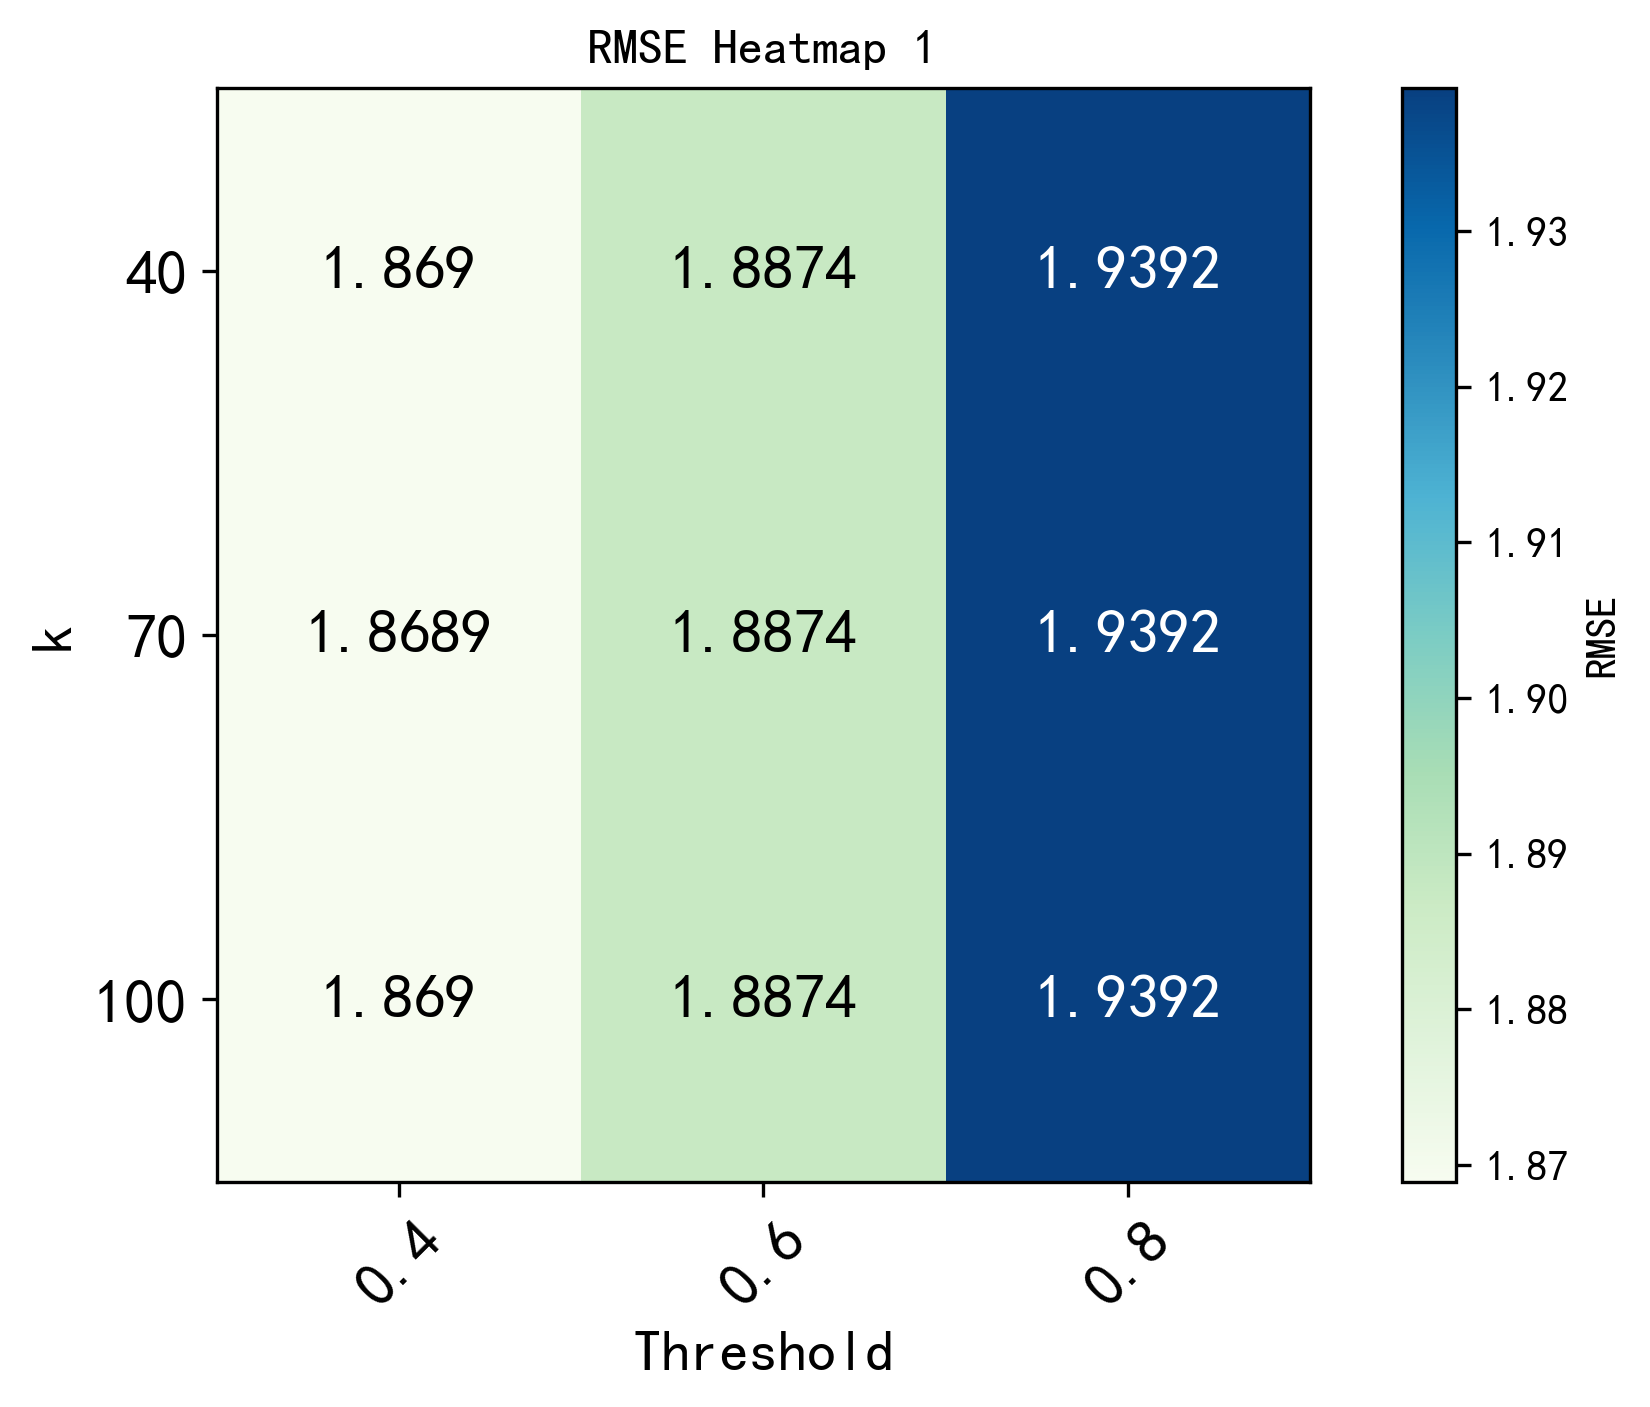
\includegraphics[width=2.5in]{Confusion_Matrix_1.png}
    }
    \subfigure[实验1的RMSE折线图]{
	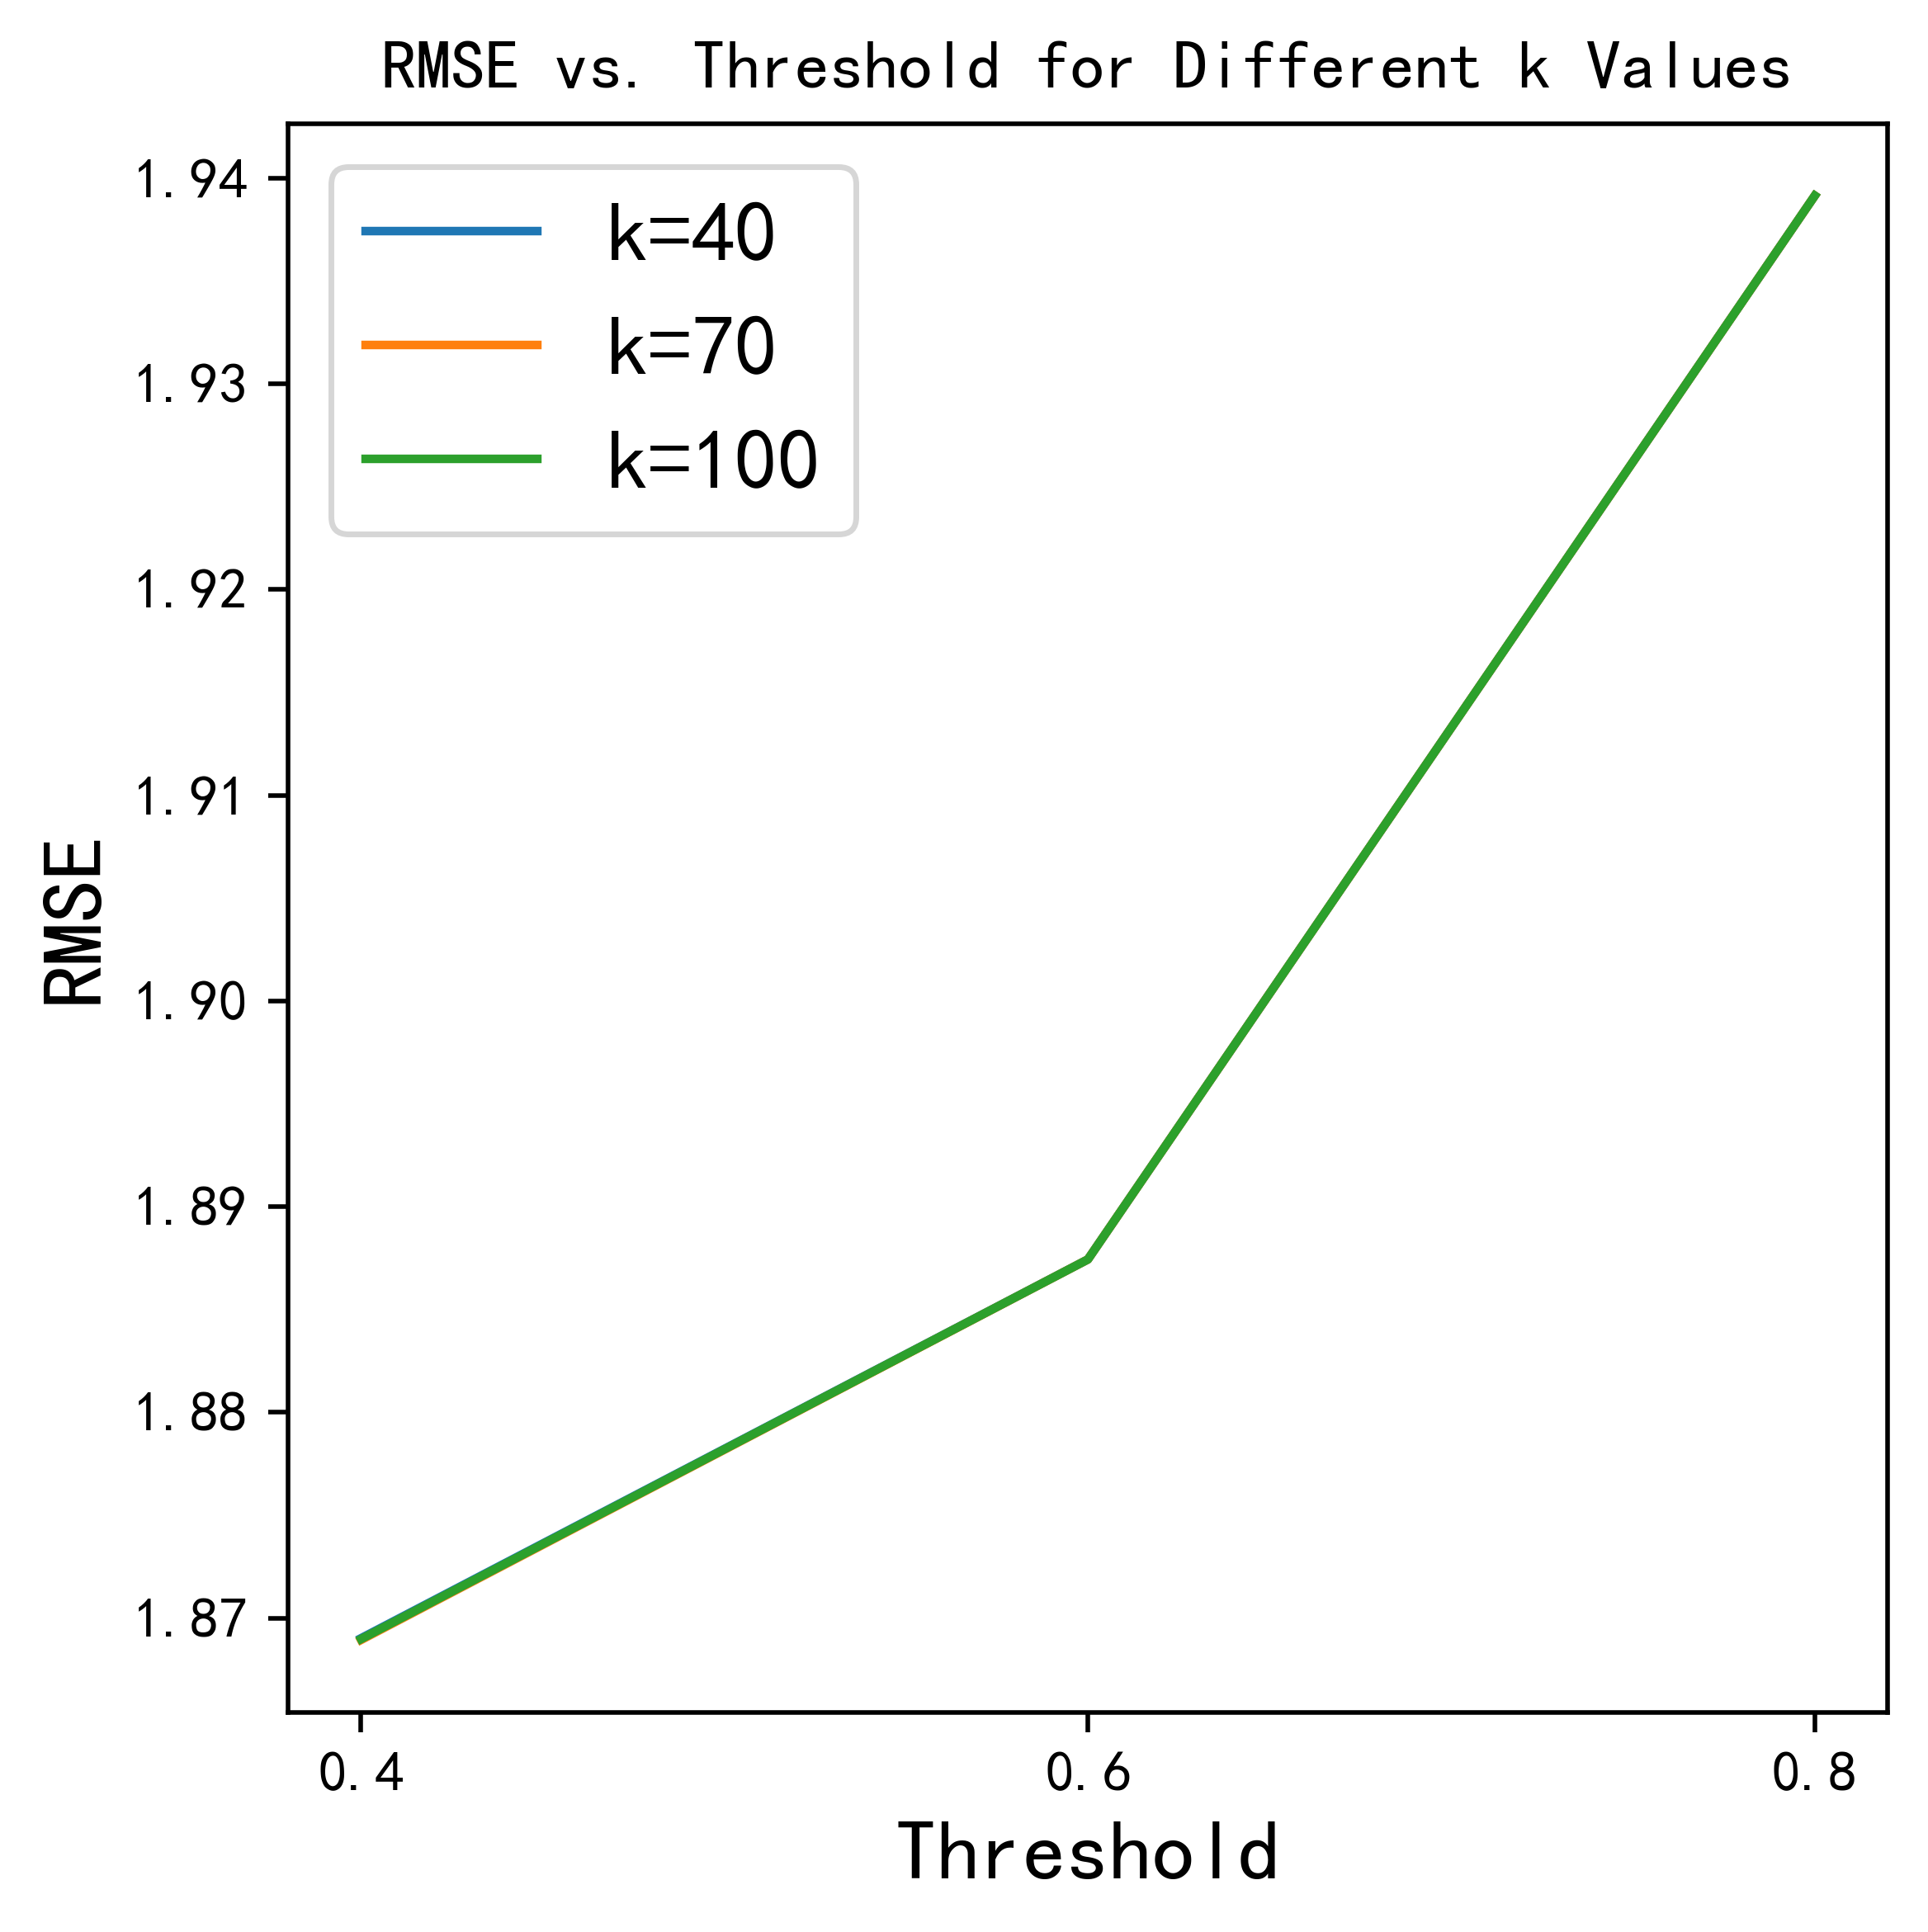
\includegraphics[width=2.15in]{Lines_1.png}
    }
    \caption{user-based CF实验1}
    \label{fig.1}
\end{figure}

\begin{figure}[htbp]
    \centering
    \subfigure[实验2的RMSE热力图]{
    	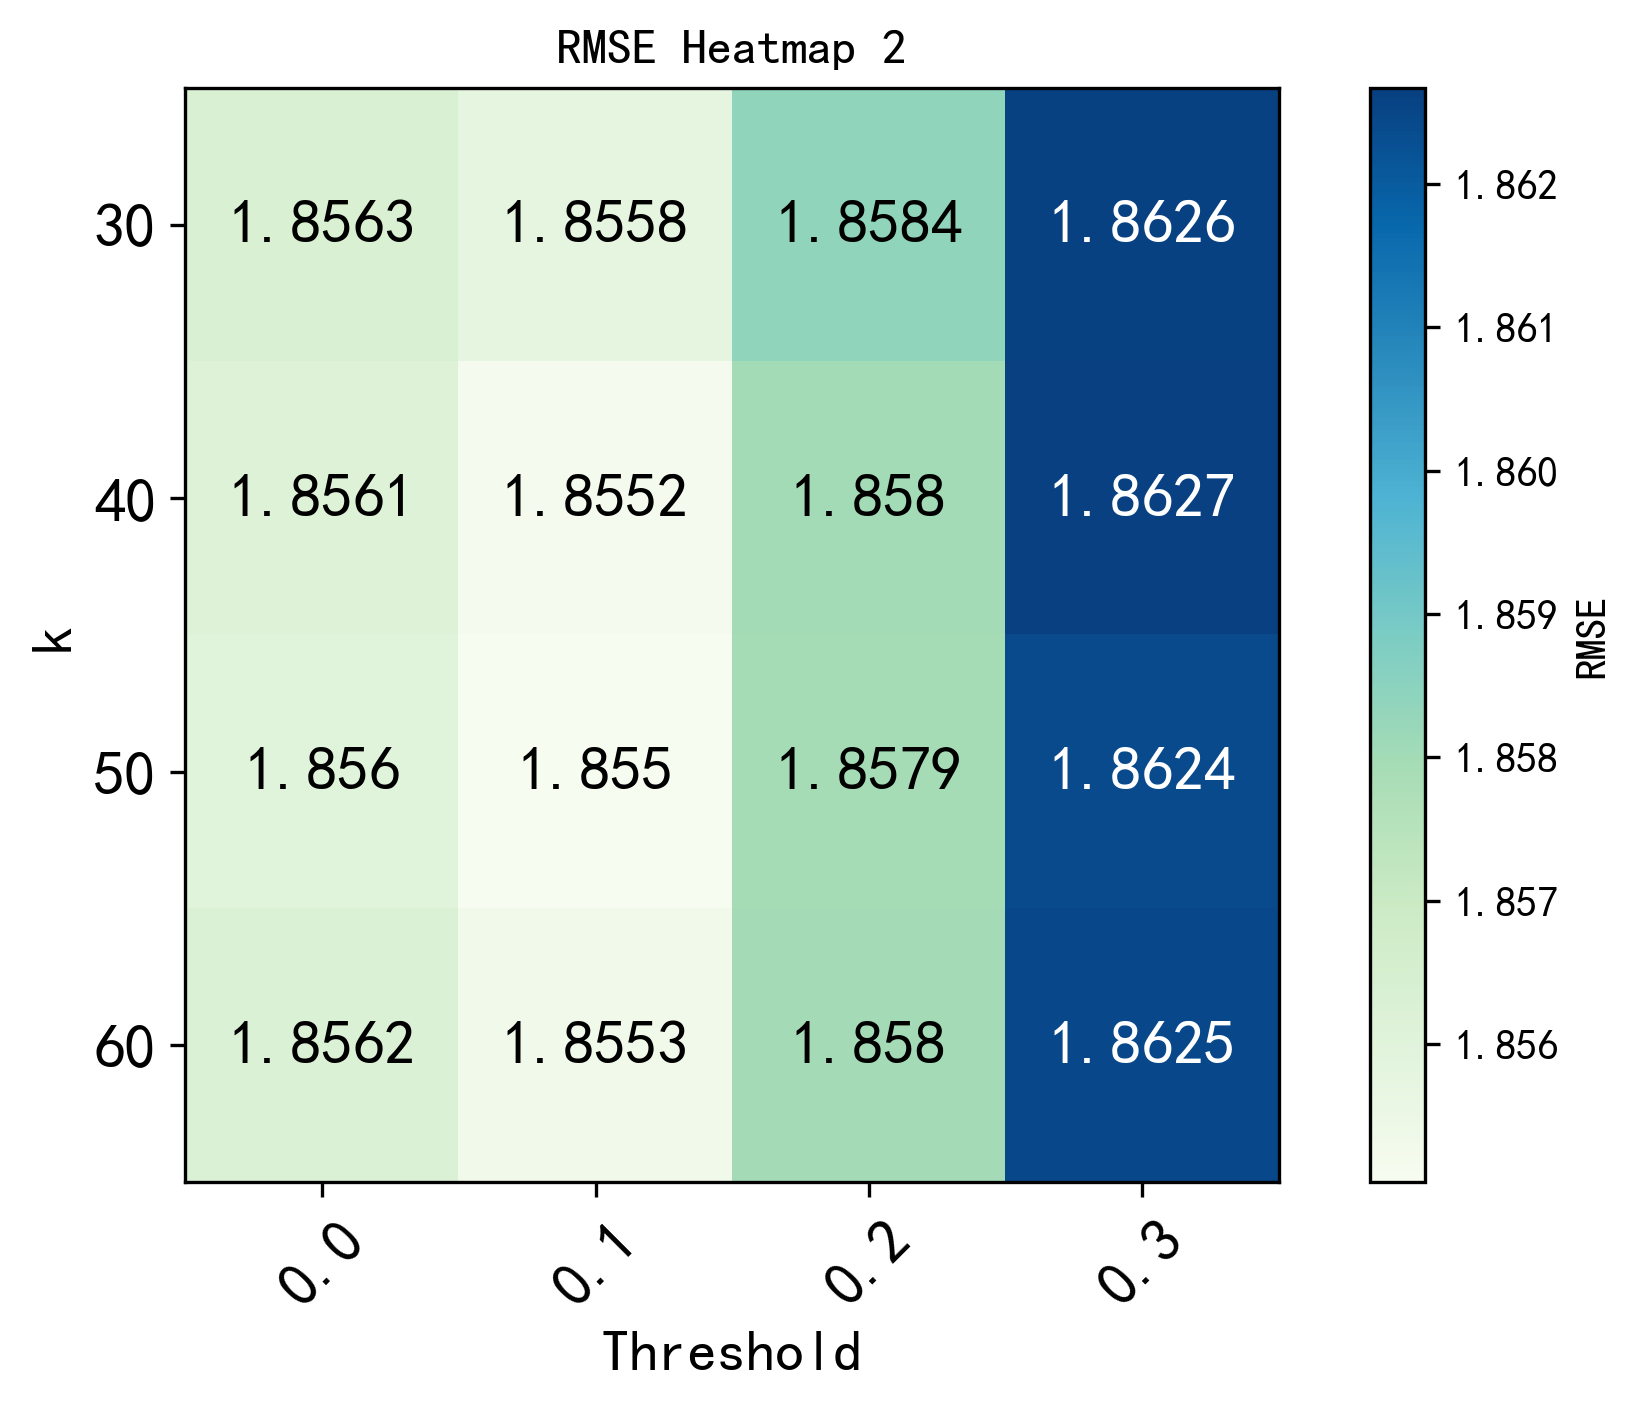
\includegraphics[width=2.5in]{Confusion_Matrix_2.png}
    }
    \subfigure[实验2的RMSE折线图]{
	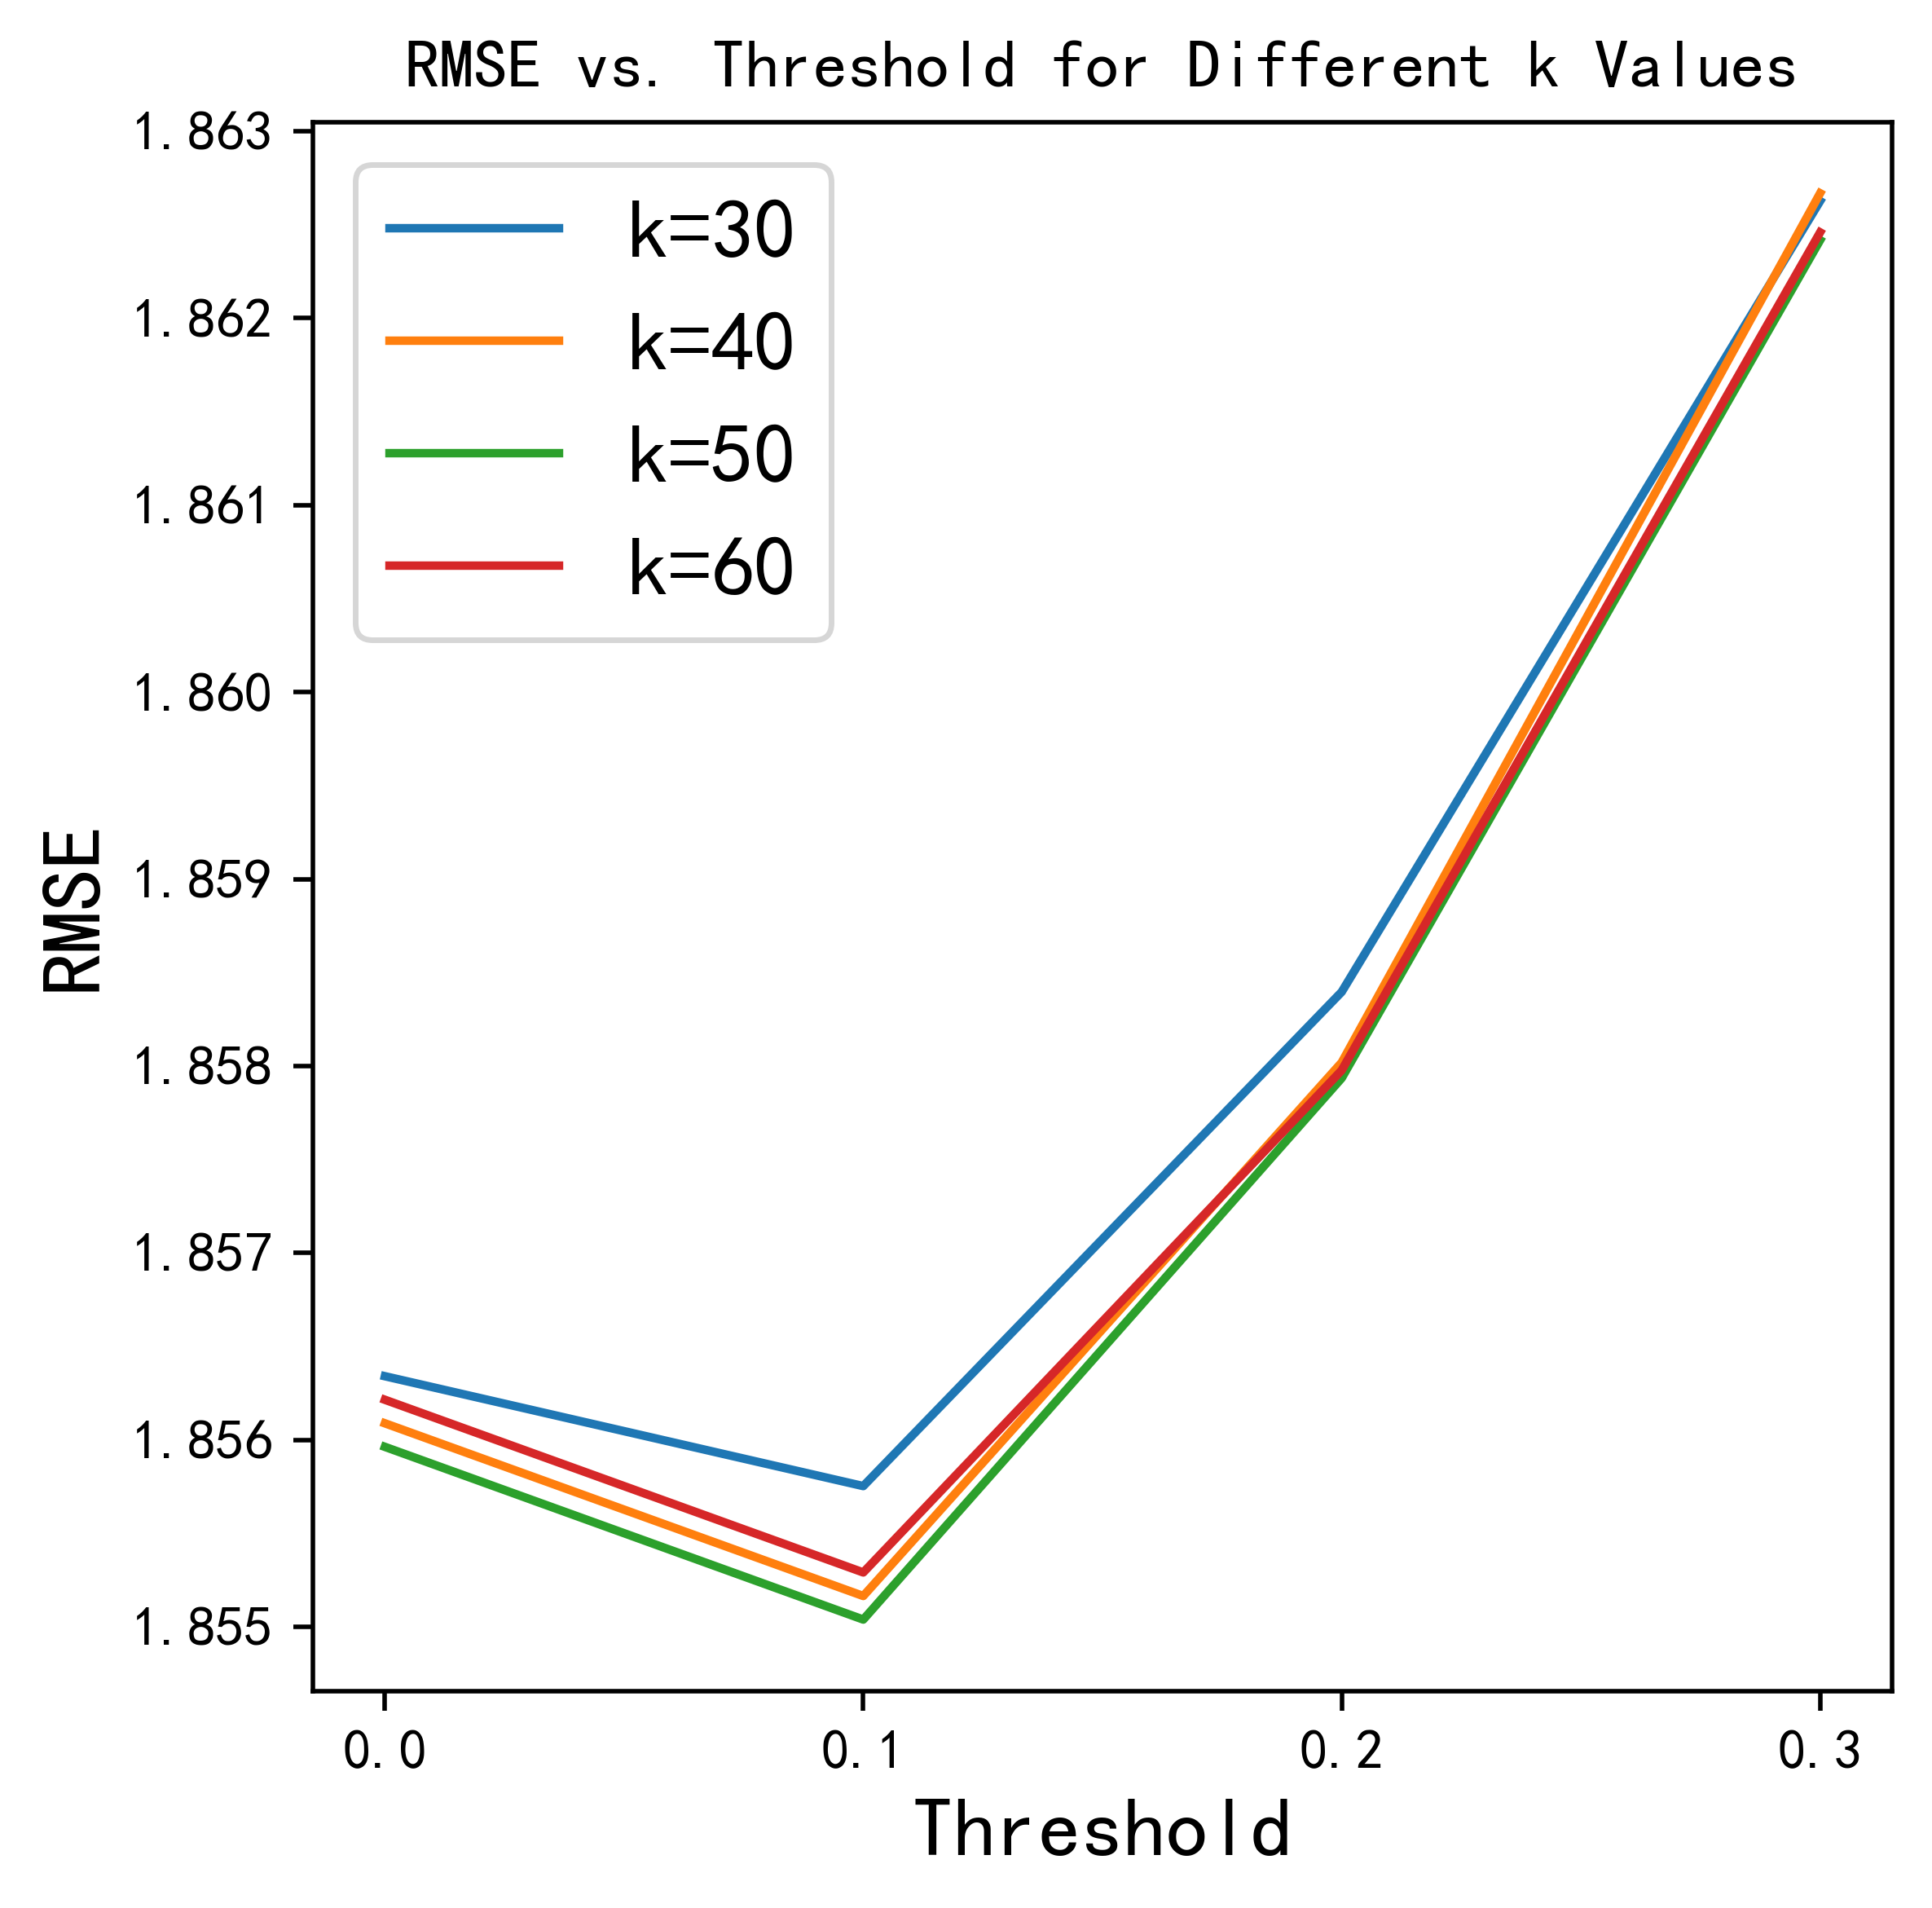
\includegraphics[width=2.05in]{Lines_2.png}
    }
    \caption{user-based CF实验2}
    \label{fig.2}
\end{figure}

\begin{figure}[htbp]
    \centering
    \subfigure[实验3的RMSE折线图]{
    	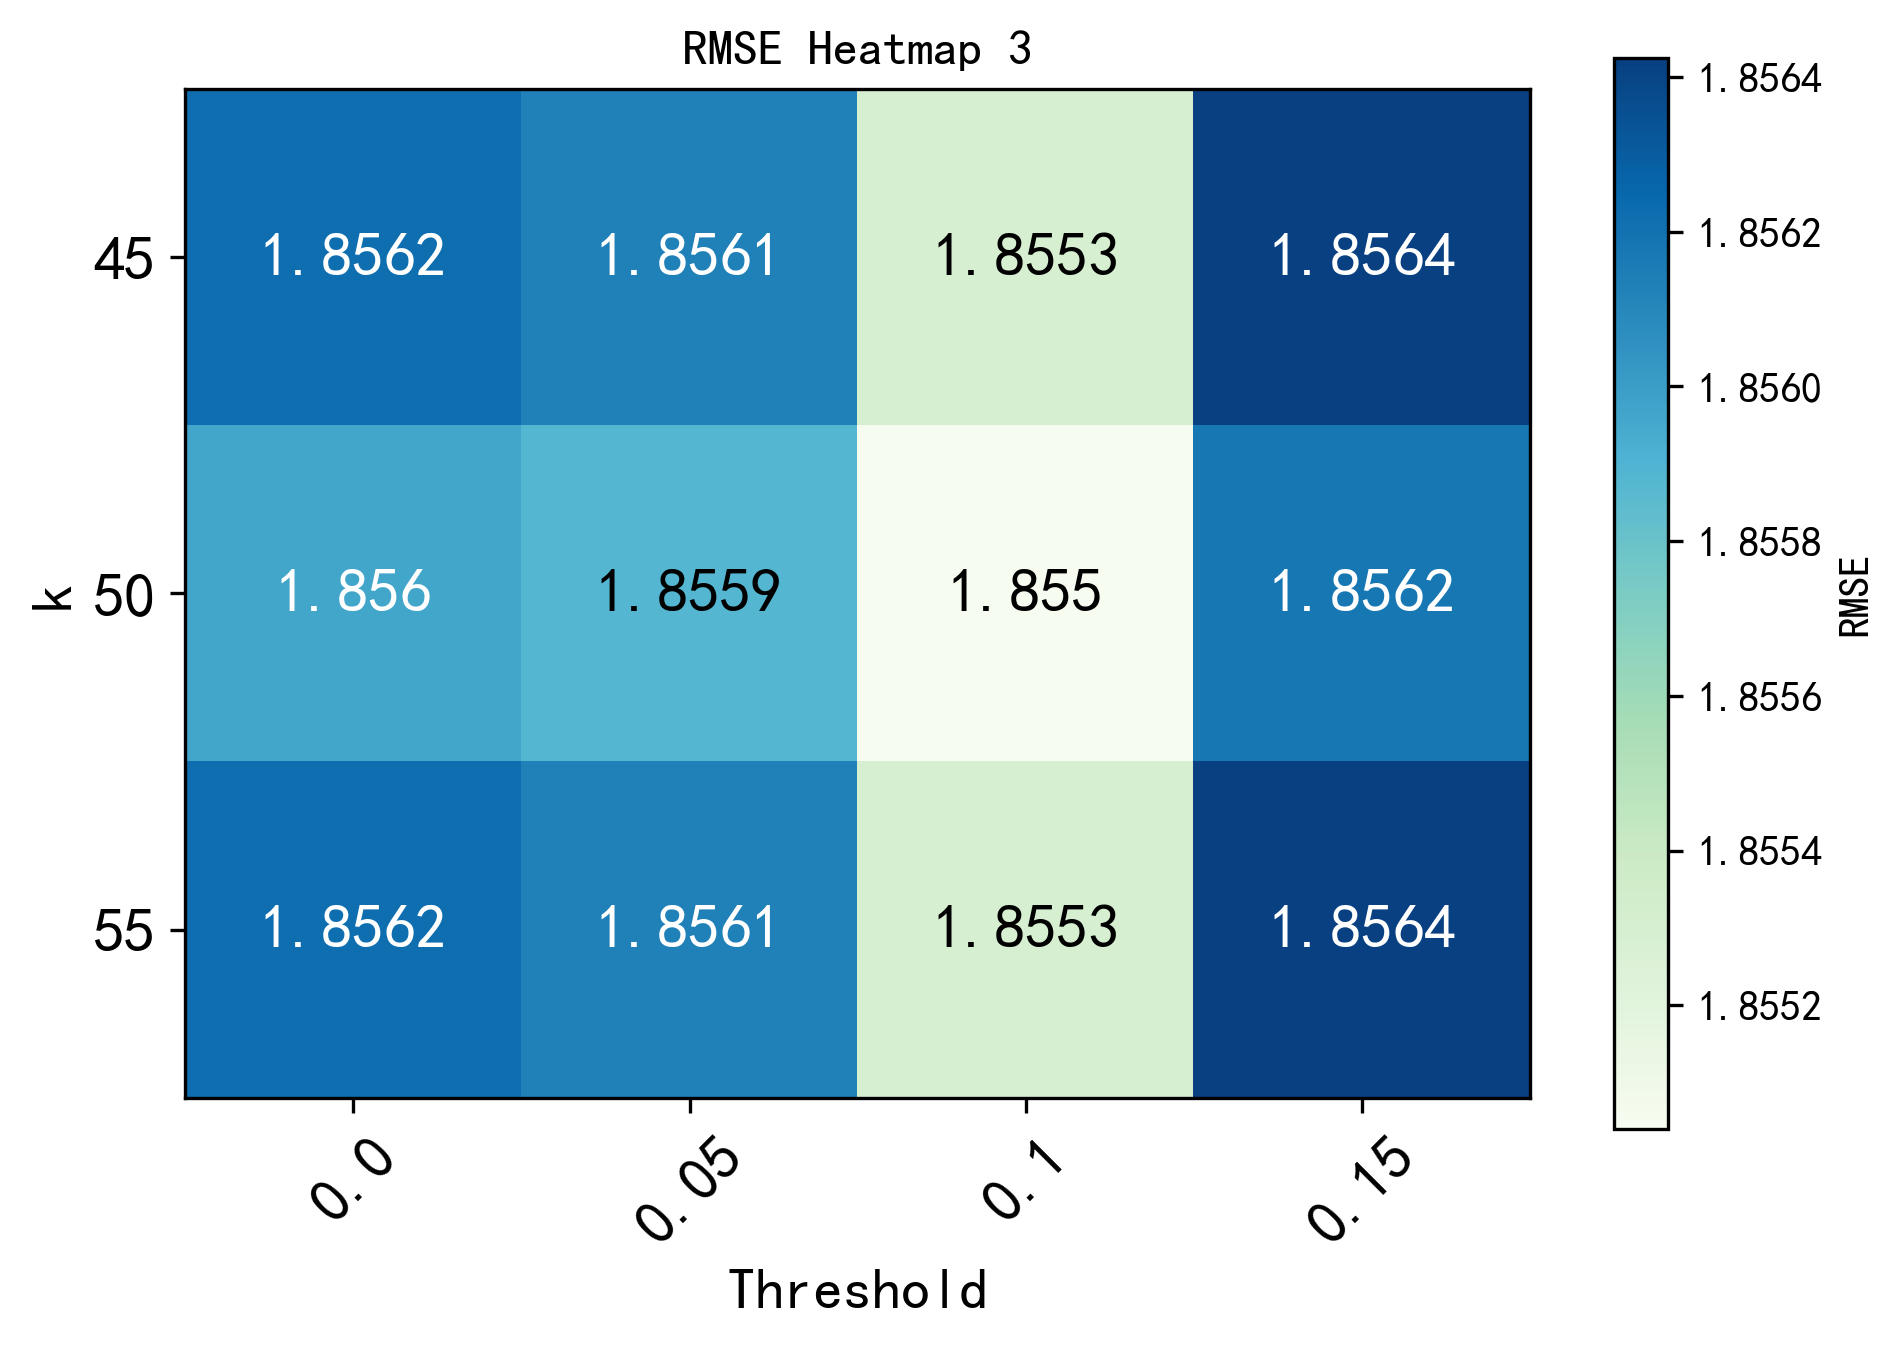
\includegraphics[width=2.6in]{Confusion_Matrix_3.png}
    }
    \subfigure[实验3的RMSE折线图]{
	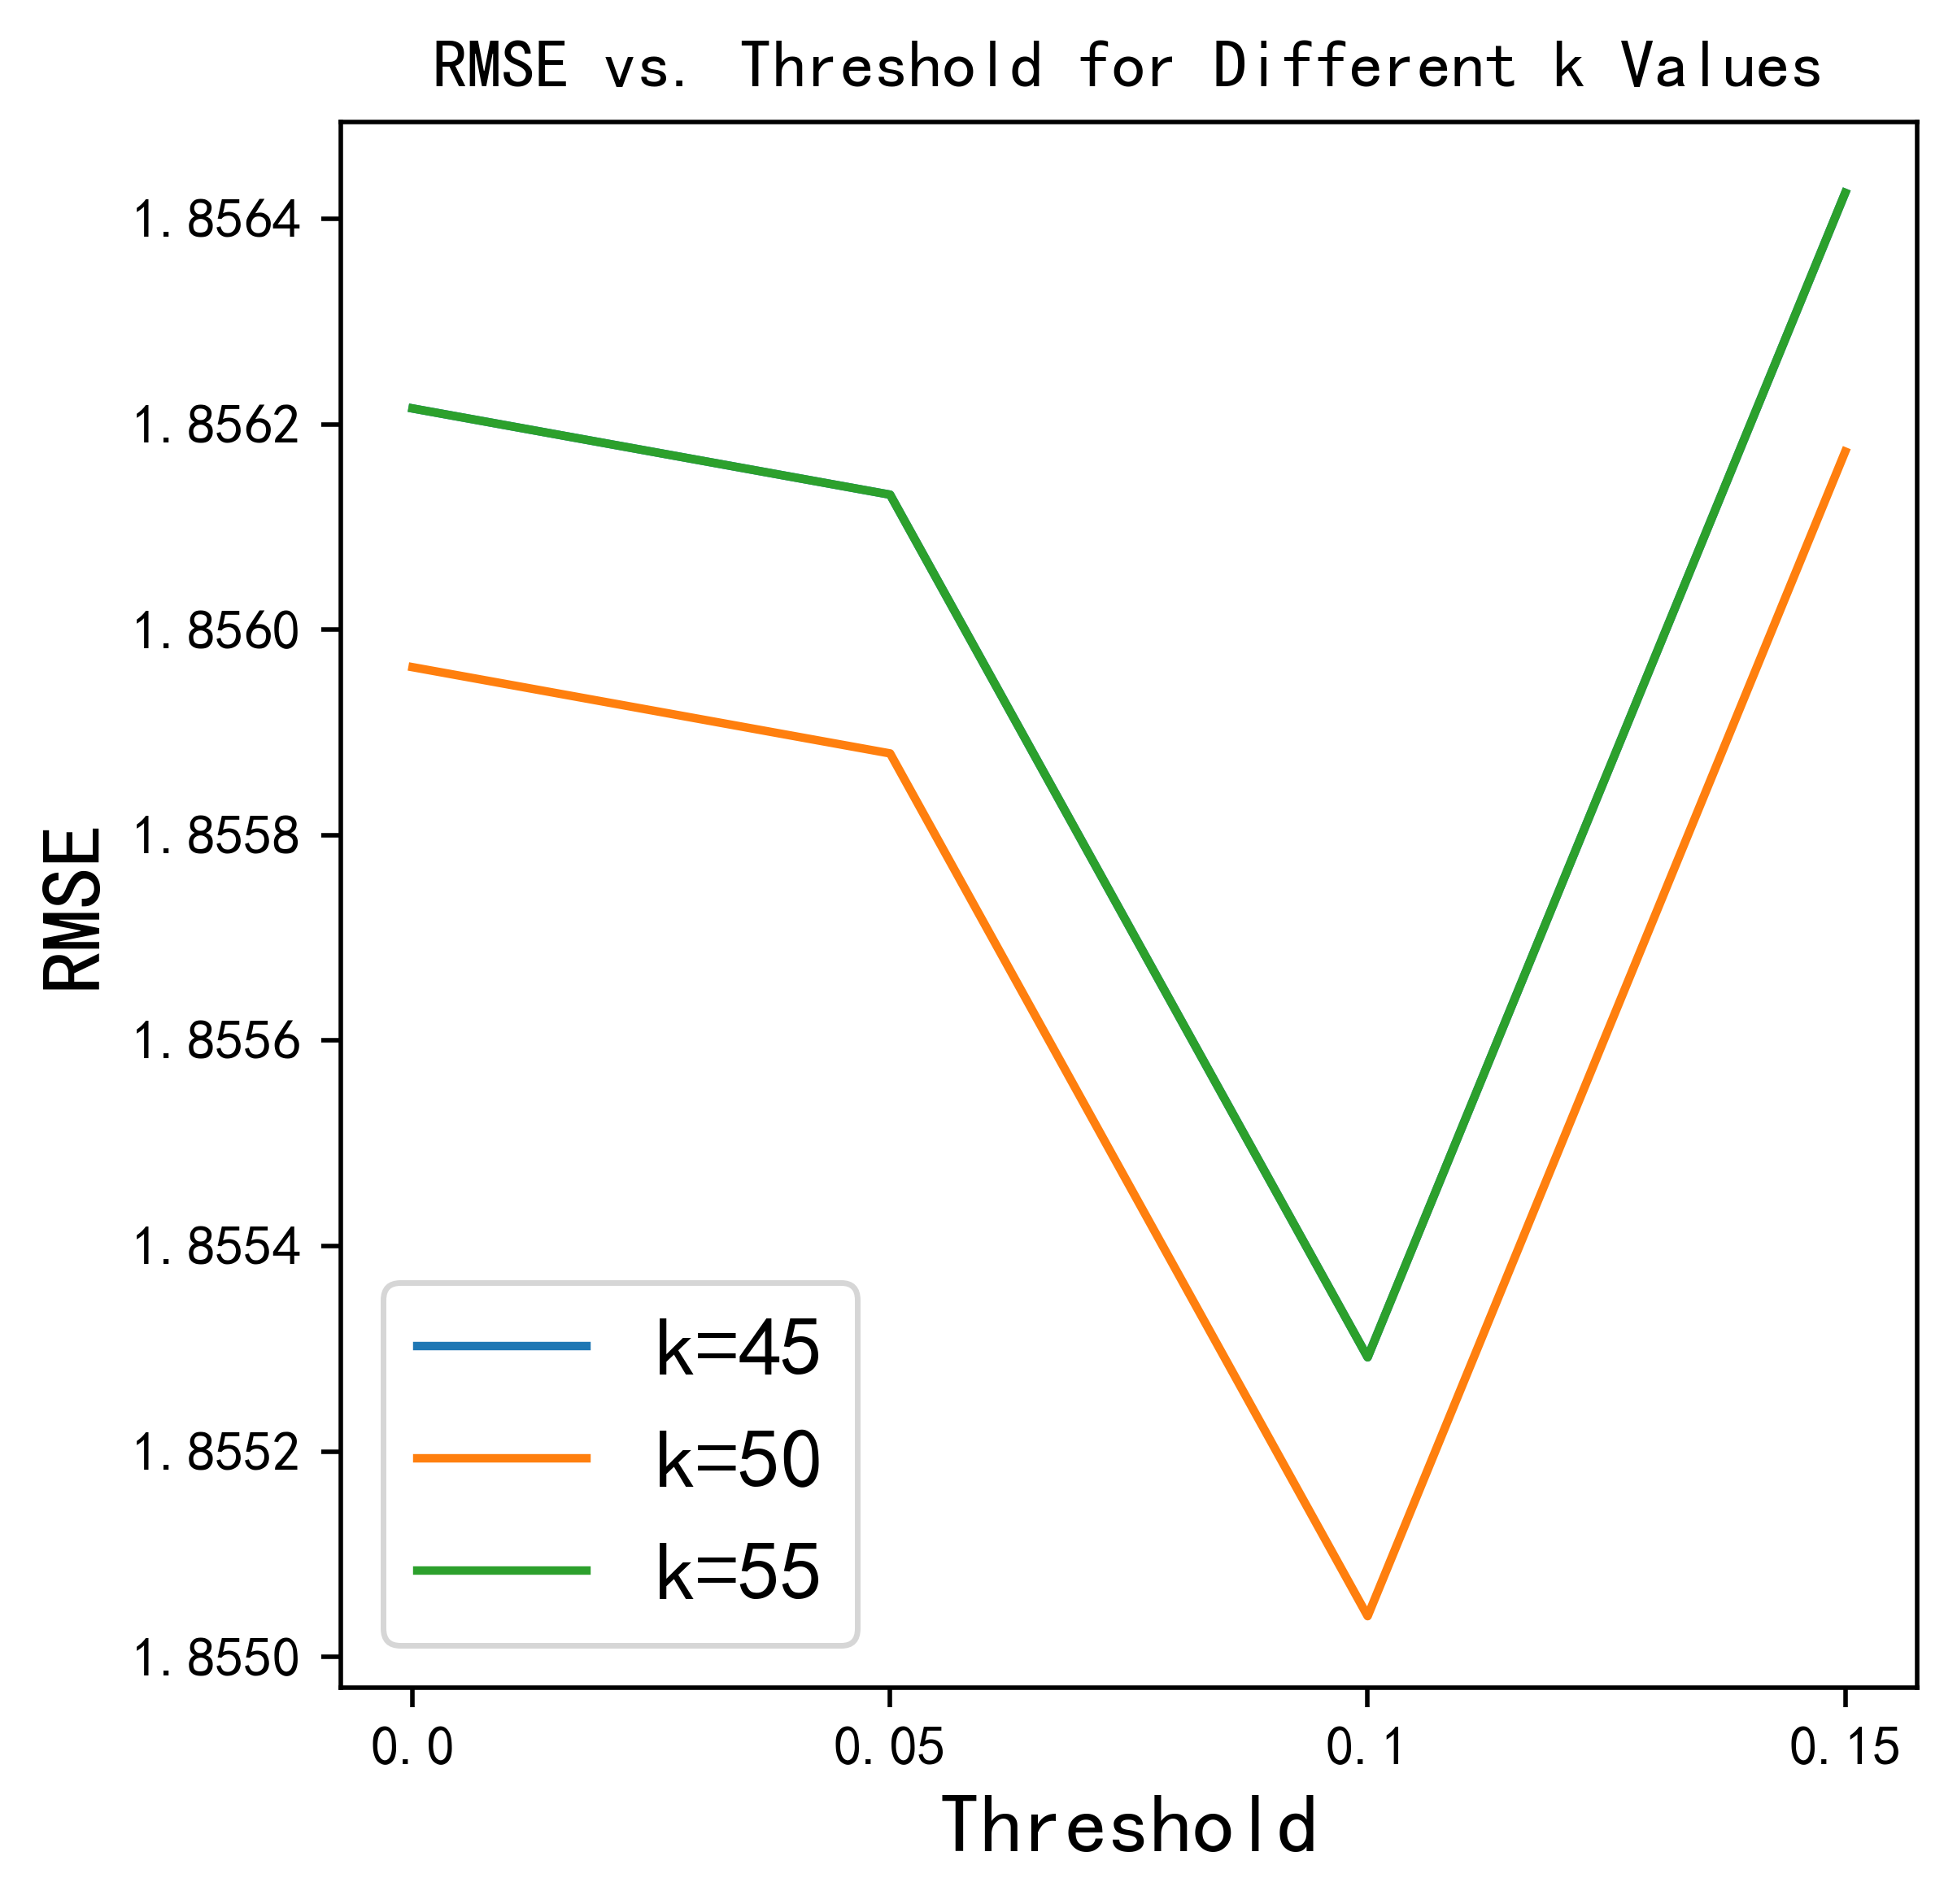
\includegraphics[width=2.0in]{Lines_3.png}
    }
    \caption{user-based CF实验3}
    \label{fig.3}
\end{figure}

接着考虑\textbf{基于物品}的协同过滤算法。设计范围比较广的实验4,从图4可见最小的RMSE也大于2,比实验1中所有RMSE都要大。简单推断知在相似度计算方法不变时,基于用户的算法总体表现更优。

\begin{figure}[htbp]
    \centering
    \subfigure[实验4的RMSE热力图]{
        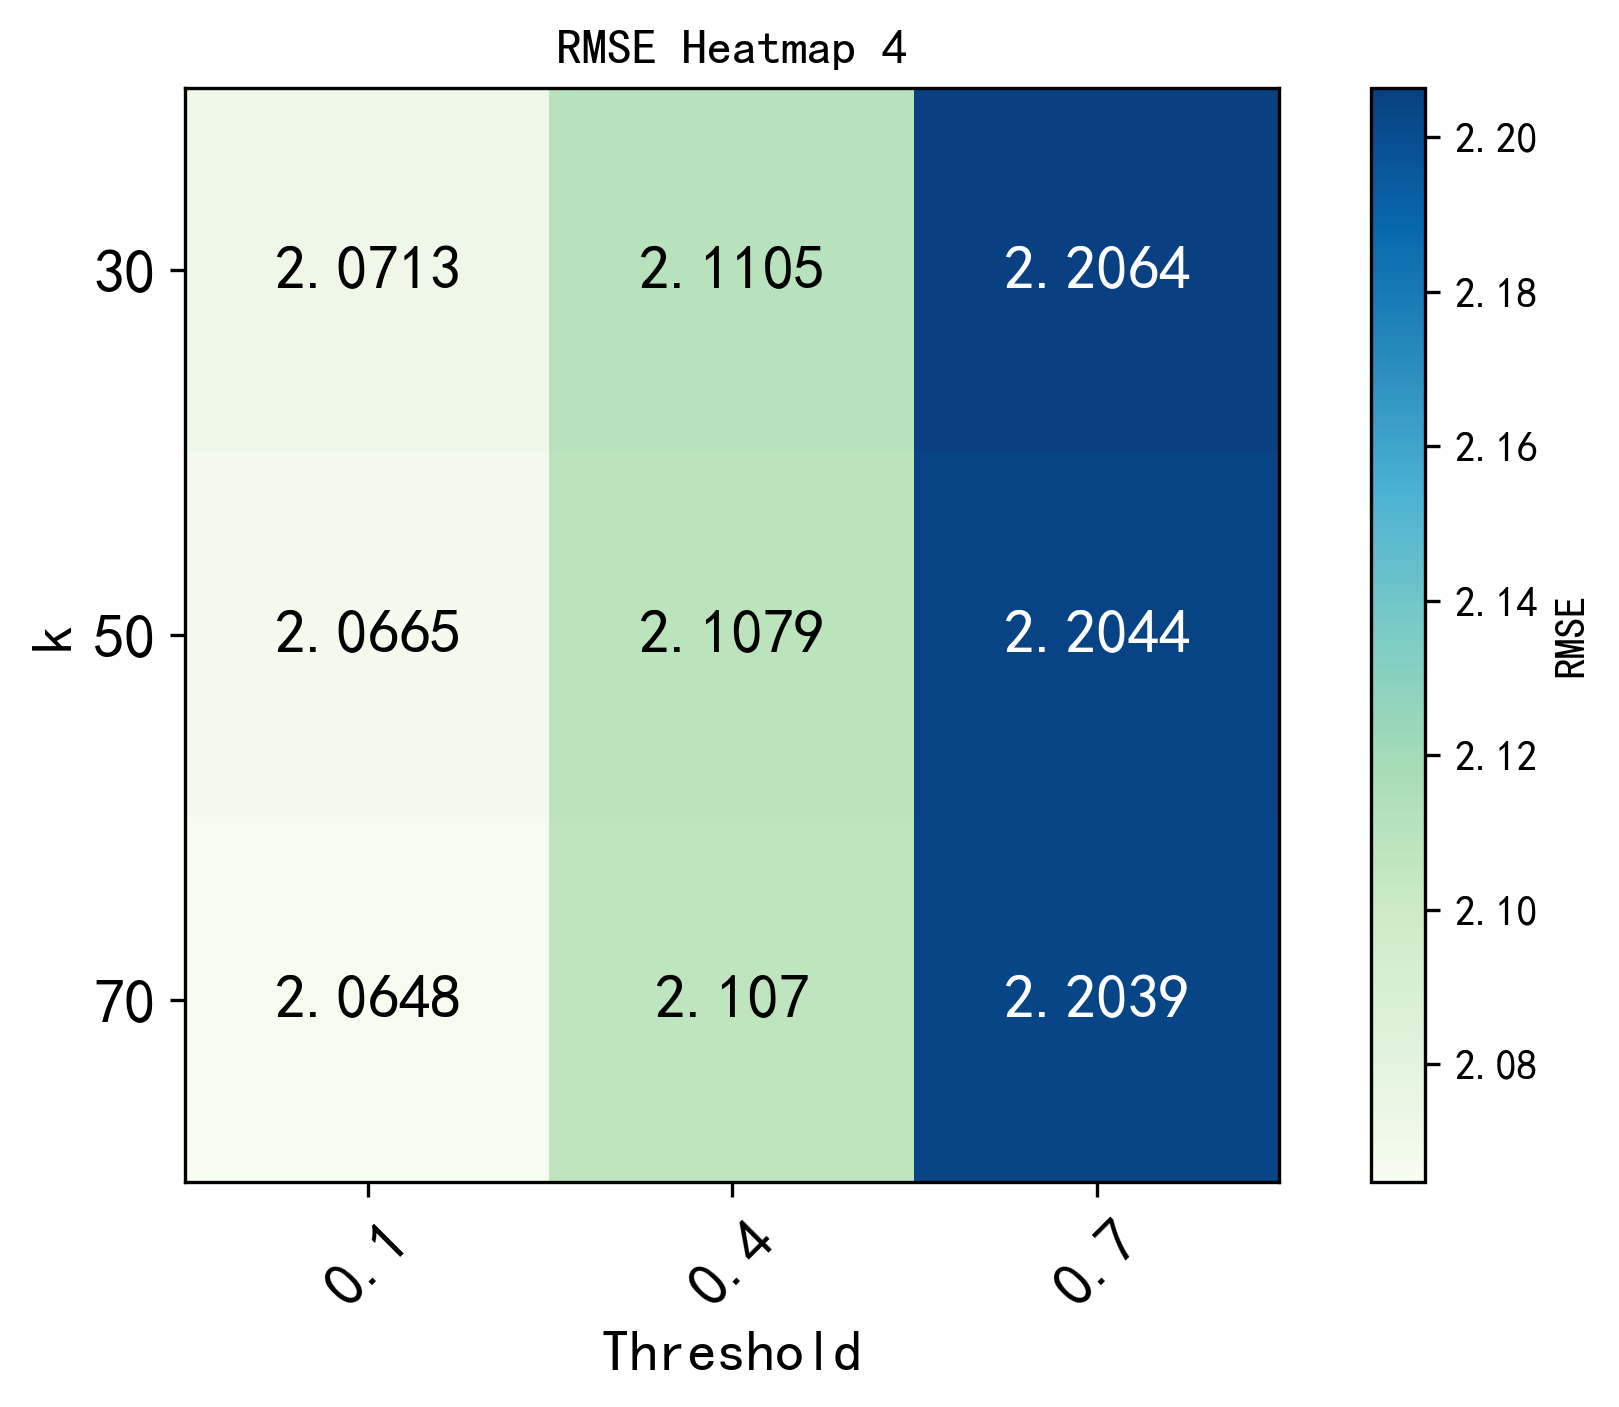
\includegraphics[width=2.5in]{Confusion_Matrix_4.png}
    }
    \subfigure[实验4的RMSE折线图]{
	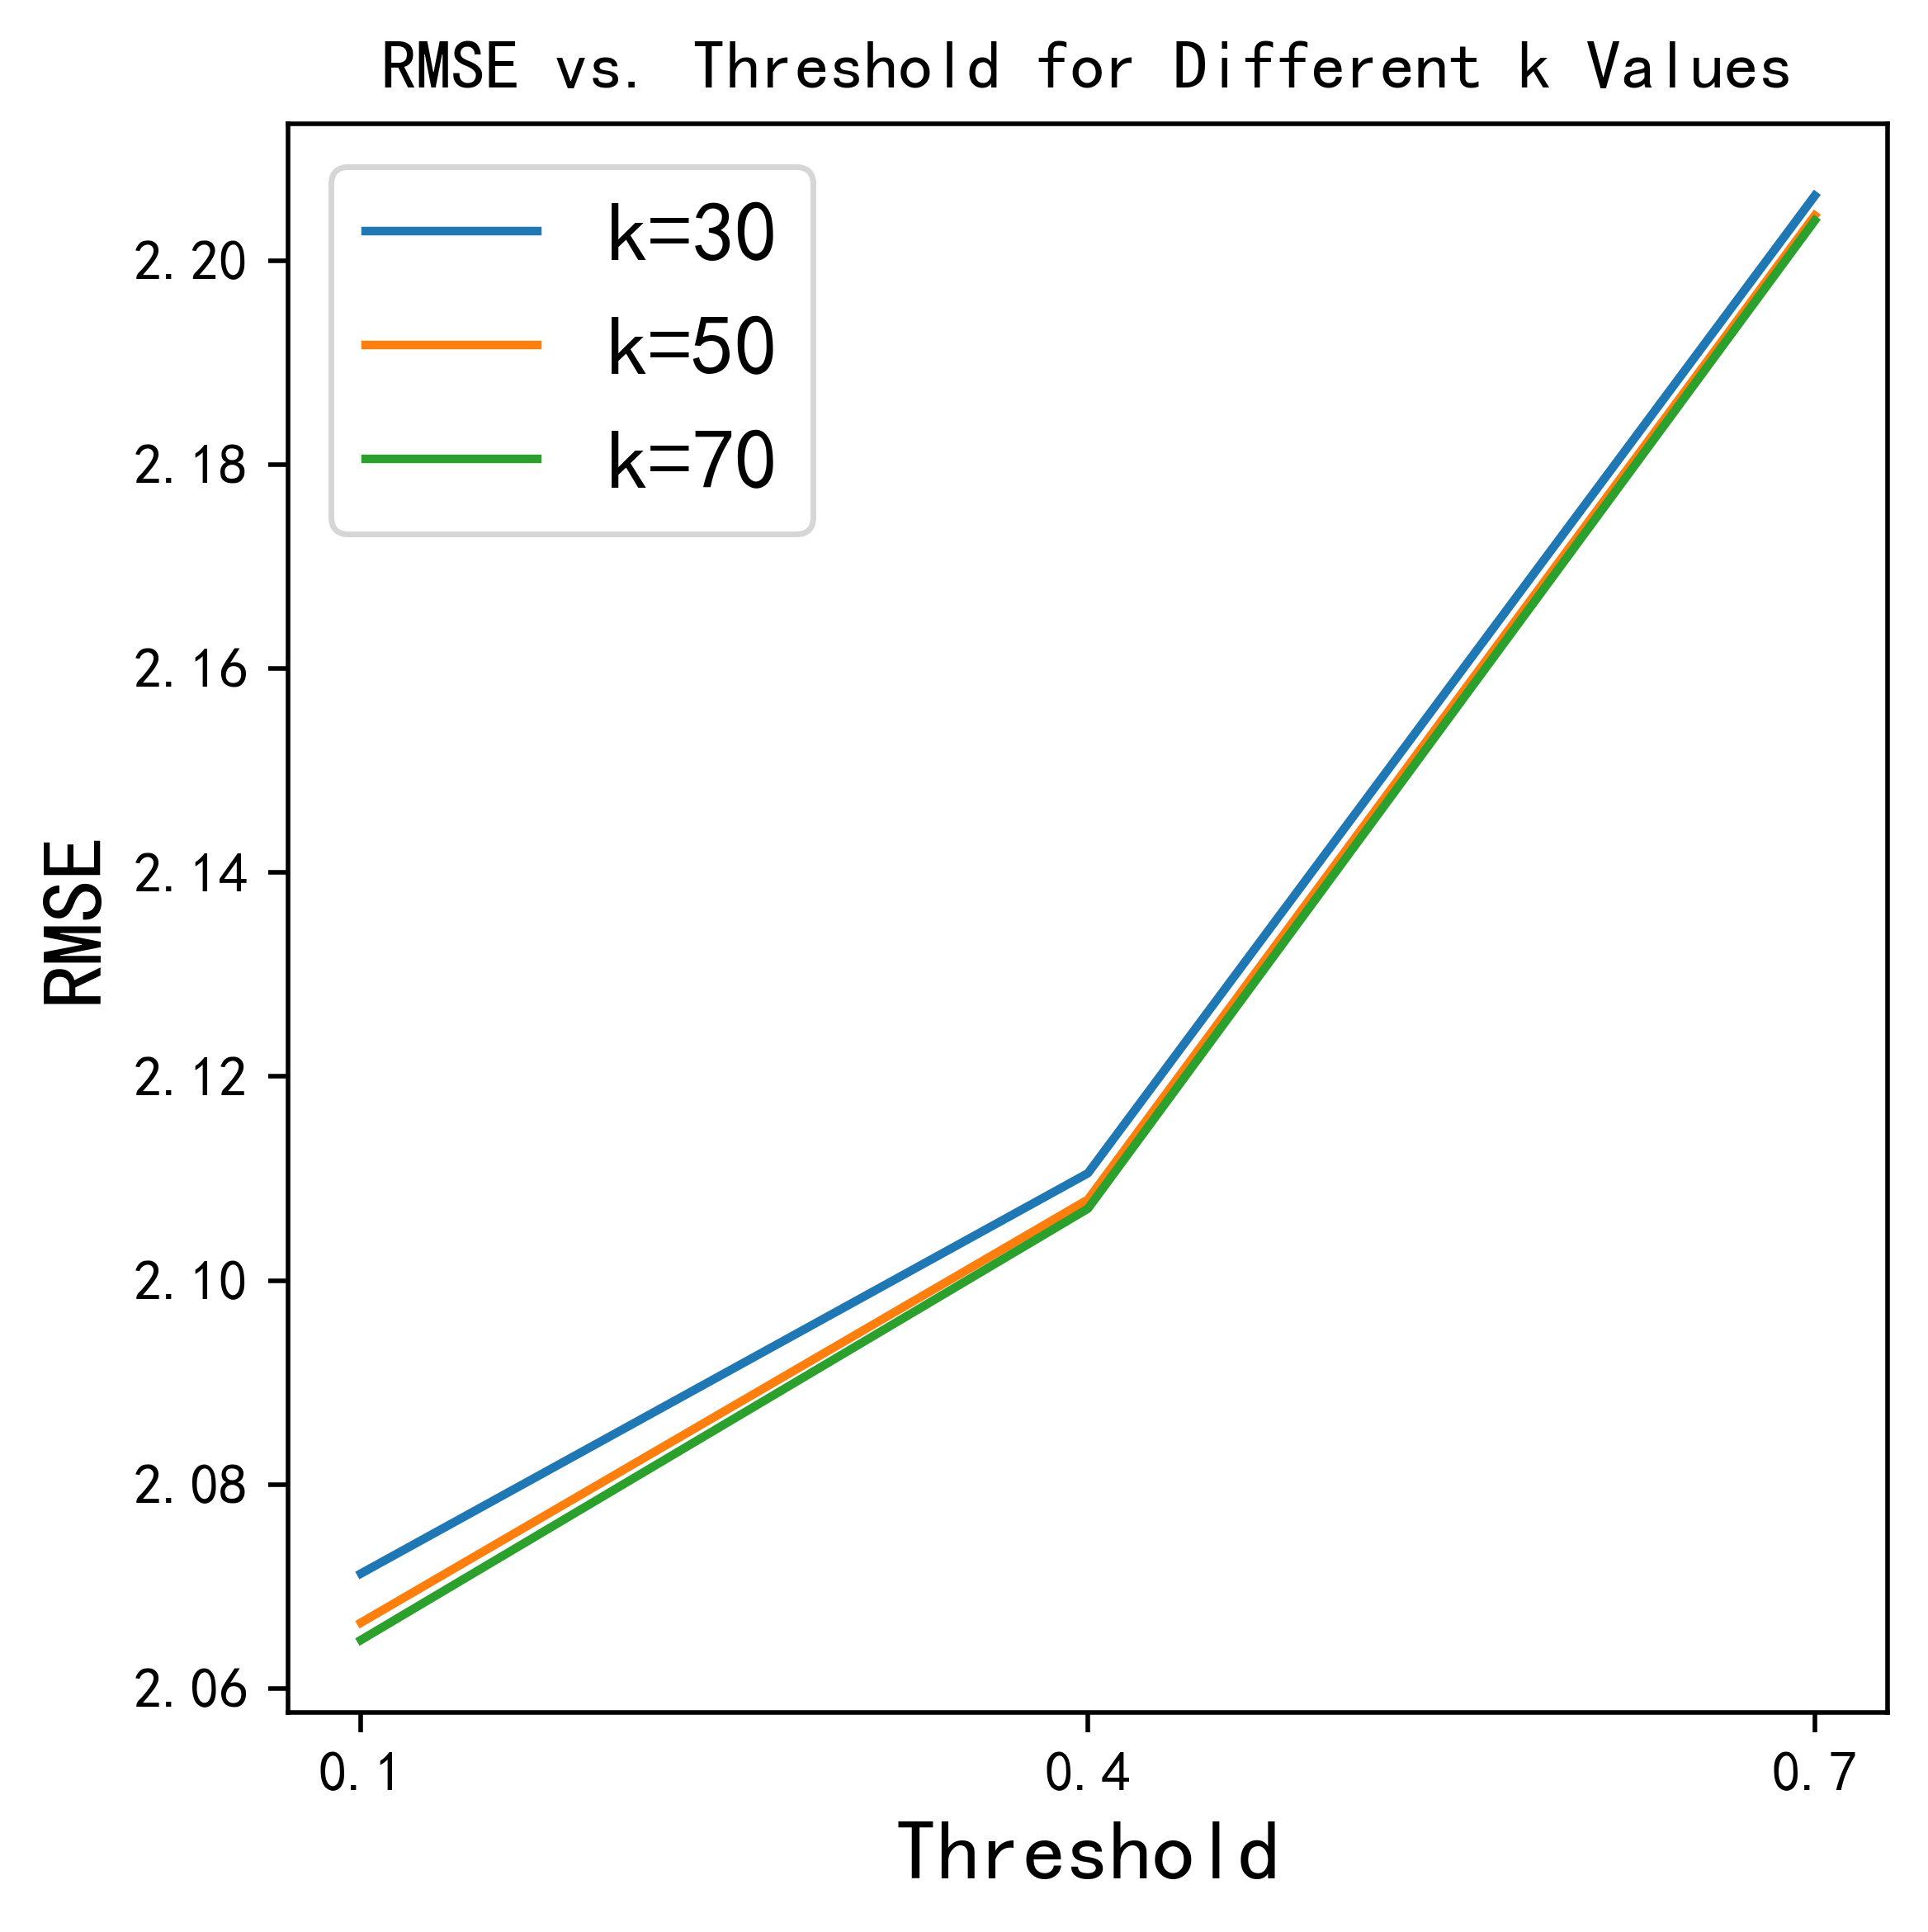
\includegraphics[width=2.15in]{Lines_4.png}
    }
    \caption{item-based CF实验4}
    \label{fig.4}
\end{figure}

综上,选择User-Based CF with Pearson Correlation,近邻集合大小K=50,相似度阈值$\lambda$=0.1.

\subsection{预测结果}

使用上一步选定好的模型,得到模型在验证集和测试集上的表现如下:
\begin{itemize}
    \item 训练数据中20\%划分为验证集时,验证集上$\hat{\rm{RMSE}}$ = 1.8550,总运行时间为49.0s.
    \item 使用完整训练数据进行训练,在测试集上$\rm{RMSE}$ = 1.83,运行时间为60.9s.
\end{itemize}

\section{提交文件列表}

压缩包\verb|`宋朝芸_10215001419_1`|包含以下这些内容:

\begin{lstlisting}
project_report.pdf

prediction_results
     output_2.csv

source_code
     Confusion_Matrix_1.png  # 第1-4次实验的在验证集上的RMSE热力图
     Confusion_Matrix_2.png  #
     Confusion_Matrix_3.png  #
     Confusion_Matrix_4.png  #
     Lines_1.png             # 第1-4次实验的在验证集上的RMSE折线图
     Lines_2.png             #
     Lines_3.png             #
     Lines_4.png             #
     output_2.csv            # 测试集上预测结果
     rmse1.csv               # 第1-4次实验的在验证集上的RMSE矩阵
     rmse2.csv               # 
     rmse3.csv               # 
     rmse4.csv               # 
     source_code.ipynb       # 源代码,jupyter notebook形式
     test.csv                # 训练数据文件
     train.csv               # 测试数据文件
\end{lstlisting}




\newpage



\end{document}
